\section{Irrationally Indifferent Fixed Points}
\sectiontitleframe
%\sectiontitleframe{Cremer Points and Siegel Discs}

\subsection{Cremer's non-linearisation theorem}
\begin{frame}{Local Linearisation}
$\lambda = e^{2\pi i \xi}$ where $\xi \in [0,1)$ is irrational.
    \begin{dfn}[Locally linearisable] The function $f$ above is said to be \emph{locally linearisable} if there is a local biholomorphic map $\linV$ which conjugates $f$ to a linear map:
\begin{equation}\label{eq: Schroder}
    \left(\linV^{-1} \circ f \circ \linV\right)(z) = \lambda z, \;
\end{equation}
for all $z$ in some neighbourhood of the origin.
\end{dfn}
\end{frame}

\begin{frame}
  We say an irrationally indifferent fixed point is a \textit{Cremer point} if there is no local linearisation of $f$ around the fixed point. A connected component of the Fatou set on which f is conjugate to a rotation of the unit disc is called a \emph{Siegel disc}.
 \begin{figure}
    \label{8:fig:Siegel Disc}
    \centering
    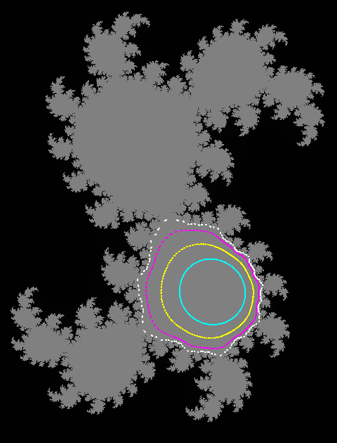
\includegraphics[width=4cm]{resources/ch-11/Picture1.png}
    \caption{Example of Siegel Disc, in white, in filled Julia set. Here, the cyan, yellow and magenta depict orbits of points nearby the origin} % <3
    
\end{figure}
\end{frame}

\begin{frame}
Main Theorems:
\begin{itemize}
    \item Cremer's Non-Linearisation Theorem
    \setbeamercovered{transparent}
    \item \onslide<2->{Siegel's Linearisation Theorem}
    \item \onslide<3->{Postcritical Closure}
\end{itemize}
\end{frame}

\begin{frame}{Cremer's Non-linearization Theorem}
    \begin{thm}(Cremer, 1938) \label{thm: 11.2}
    Given $\lambda \in \C$ on the unit circle and $d \geq 2$, if the sequence $\sqrt[d^{q}]{1 / \abs{\lambda^q - 1}}$ is unbounded as $q \tendsto \infty$, no fixed point with multiplier $\lambda$ of a rational function of degree $d$ can be locally linearisable.
\end{thm}
\end{frame}

\begin{frame}{Sketch Proof Cremer's Theorem}
Case when
\[
f(z) = z^{d} + \dots + \lambda z,  d \geq 2
\]
\begin{itemize}
    \item $f^{oq}(z) = z^{d^{q}} + \dots + \lambda^{q} z$
    \item Fixed points of $f^{oq}$ satisfy the polynomial $z^{d^{q}} + \dots + (\lambda^{q} - 1)z = 0$. Then 
    \[
    \prod_{j = 1}^{d^{q}-1} \left|{ z_{q}{(j)}}\right| = \abs{\lambda^{q} - 1}
    \]
    \item $\abs{\lambda^{q} - 1} < 1 \Longrightarrow \exists\; j_{q}$\; s.t.\;$ 0 < \left| z_{q}(j_q) \right| < \abs{\lambda^{q} - 1}^{1/d^{q}}$
    \item Sequence $(q_{k})_{k\geq 1}$ where
    \begin{align*}
    \abs{\lambda^{q_k} - 1}^{-1/d^{q_{k}}} &\tendsto \infty\\
    \implies \abs{\lambda^{q_k} - 1}^{1/d^{q_{k}}} &\tendsto 0
    \end{align*}
    \item Every neighbourhood of the origin has infinitely many periodic points
\end{itemize}
\end{frame}

\begin{frame}{Siegel's Linearization Theorem}
\begin{dfn}
For $\xi \in \R$, we say $\xi$ is \textit{Diophantine of order $\leq \kappa$} if\; $\exists\; \eps > 0$ such that
\[
\abs{\xi - \frac{p}{q}} > \frac{\eps}{q^{\kappa}}
\]
for any rational $\frac{p}{q}$
\end{dfn}

Certainly Diophantine of order $\leq \kappa \Longrightarrow$ Diophantine of order $\leq \kappa + 1$

\begin{lem}
With $\xi$ as above, $\xi$ is Diophantine of order $\leq \kappa \Longleftrightarrow$ there exists $M > 0$ such that $\forall\; q \in \Z_{\geq 1}$
\[
1/\abs{\lambda^{q}-1} < Mq^{\kappa - 1}
\]
\end{lem}
\end{frame}

\begin{frame}{Siegel's Linearization Theorem}
\begin{thm}
If the angle $\xi$ is Diophantine of any order, then any
holomorphic germ with multiplier $\lambda = e^{2\pi i\xi}$ is locally linearisable. Hence, if there exists $M > 0$ and $k \in \N$ such that $\forall\; q \in \Z_{\geq 1}$
\[
1/\abs{\lambda^{q}-1} < Mq^{k}
\]
then any holomorphic function with a fixed point of multiplier $\lambda$ is locally linearisale.
\end{thm}
\begin{cor}
In terms of the Lebesgue measure on $[0,1)$, almost every $\xi$ has the property that any holomorphic function with fixed point of multiplier $e^{2\pi i \xi}$ is locally linearizable. 
\end{cor}
\end{frame}

\begin{frame}{Generic vs Lebesgue Almost Everywhere}
    \begin{itemize}
        \item Cremer: for a \textit{generic} choice of angle $\xi$, there exists a holomorphic function with fixed point of multiplier $\lambda = e^{2\pi i \xi}$ which is not locally linearizable.
        \item Siegel: for \textit{almost every} angle $\xi$, any holomorphic function with fixed point of multiplier $\lambda = e^{2\pi i \xi}$ is locally linearizable.
    \end{itemize}
    
     \par\vspace{1em}
     
    \textit{A linguist would be shocked to learn that if a set is not closed this does not mean that it is open, or again that “E is dense in E” does not mean the same thing as “E is dense in itself"}
    
     \par\vspace{1em}
    % Yeah I latex
    % D:<
    - John Edensor Littlewood (1885–1977)
\end{frame}




















